\begin{rep}
En posant
%\begin{eqnarray*}
$\bar{x}_n  =  \frac{1}{n}\sum\limits_{i=1}^n x_i$ et 
$\bar{b}_{{\bf x_n}}(\lambda)  =  \sum\limits_{i=1}^n \exp\left(-\lambda x_i\right)$, 
la vraisemblance s'écrit alors
\begin{eqnarray*}
f\left({\bf x_n}\right) & = & \lambda^n \mu^n \exp(-\lambda n\bar{x}_n) \exp\{-\mu\bar{b}_{{\bf x_n}}(\lambda)\}.
\end{eqnarray*}
En conséquence, la loi {\it a posteriori} s'obtient sous la forme \emph{hiérarchisée} suivante :
\begin{eqnarray*}
\pi\left(\mu,\lambda|{\bf x_n}\right) & = & \pi\left(\mu|\lambda,{\bf x_n}\right) \pi\left(\lambda|{\bf x_n}\right)
\end{eqnarray*}
où
\begin{eqnarray*}
\mu|\lambda,{\bf x_n} & \sim & {\cal{G}}\left(m+n,b_m(\lambda) + \bar{b}_{{\bf x_n}}(\lambda)\right)
\end{eqnarray*}
et
\begin{eqnarray*}
\pi\left(\lambda|{\bf x_n}\right) & =  & %\underbrace{\propto}_{\text{\tiny proportionnel}} &  
\gamma(\lambda)\cdot {\cal{G}}\left(m+n,{m}/{\lambda_e} + n\bar{x}_n\right)
%\frac{\left(b_m(\lambda)\right)^m}{\left(b_m(\lambda) + \bar{b}_{{\bf x_r},{\bf c_{n-r}}}(\lambda)\right)^{m+r}} \lambda^{m+r-1} \exp\left(-\lambda ({m}/{\lambda_e} + r\bar{x}_r) \right)
\end{eqnarray*}
avec
\begin{eqnarray*}
\gamma(\lambda) & \propto & \frac{b^m_m(\lambda)}{ \left(b_m(\lambda) + \bar{b}_{{\bf x_n}}(\lambda)\right)^{m+n}}
\end{eqnarray*}
La loi {\it a priori} est donc \emph{semi-conjuguée}, et il suffit de simuler $\lambda$ {\it a posteriori} pour obtenir un tirage joint {\it a posteriori} de $(\mu,\lambda)$. On trace ci-dessous quelques graphiques typiquement obtenus. Plusieurs choix de lois instrumentales pour $\rho(\lambda|\lambda^{(i-1)})$ peuvent être faits. On peut notamment proposer : 
\begin{itemize}
\item la loi {\it a priori} $\pi(\lambda)$ ; 
\item une loi qui ``semble proche": ${\cal{G}}\left(m+n,{m}/{\lambda_e} + n\bar{x}_n\right)$ ; 
\item une loi normale de moyenne $\lambda^{(i-1)}$ et de coefficient de variation petit (5\%) ou grand (25 ou 50\%).
\end{itemize}


\begin{center}
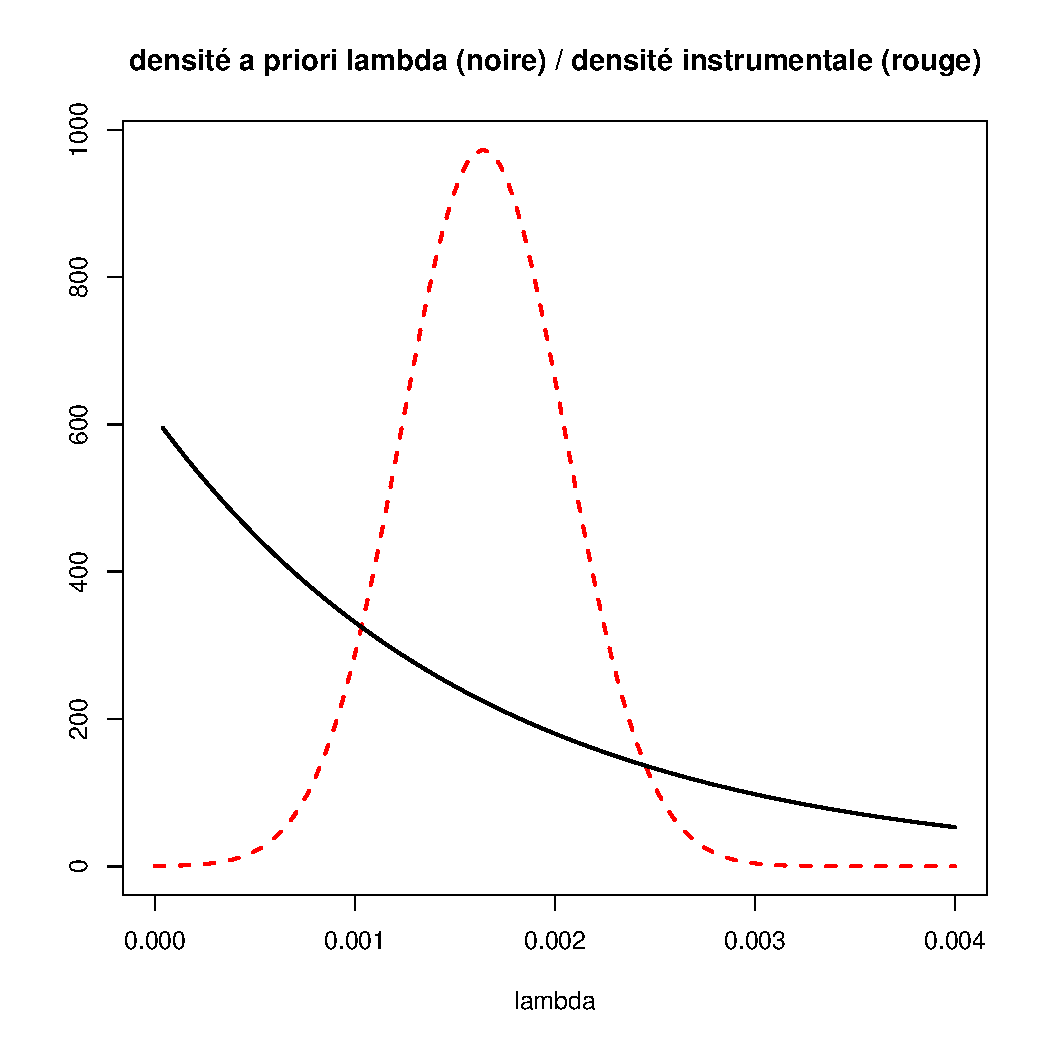
\includegraphics[width=6cm,height=5cm]{figures/calcul/prior-1.pdf} 
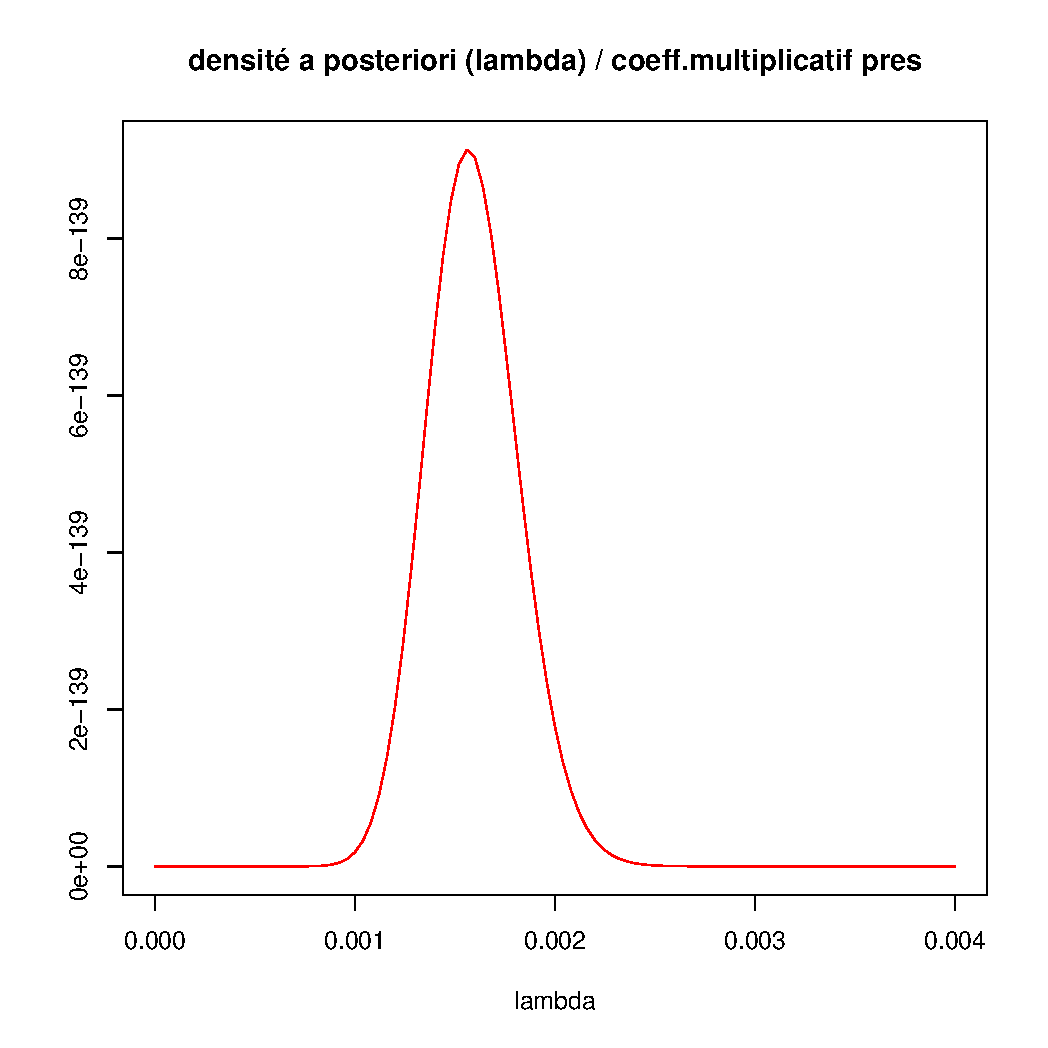
\includegraphics[width=6cm,height=5cm]{figures/calcul/posterior-1.pdf} \\
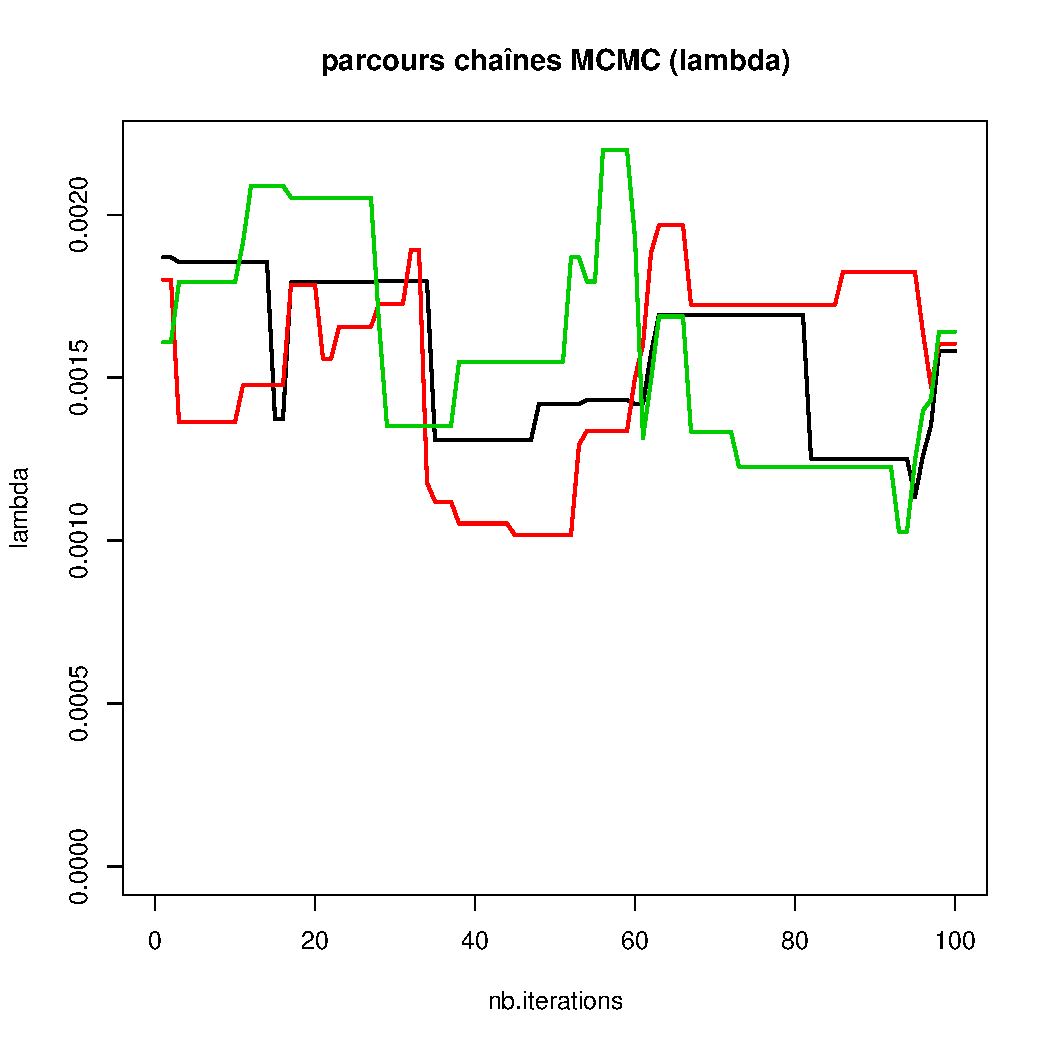
\includegraphics[width=6cm,height=5cm]{figures/calcul/MCMC1.pdf}
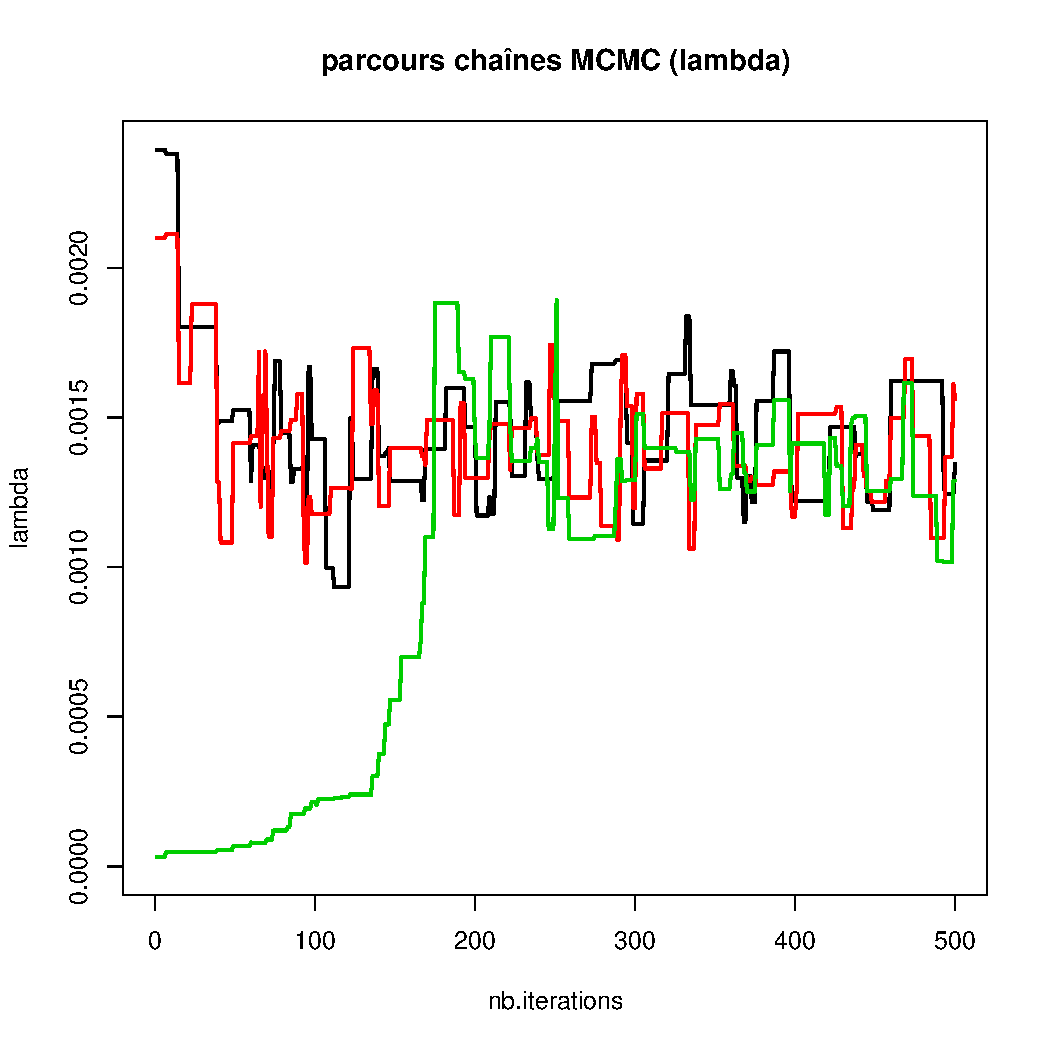
\includegraphics[width=6cm,height=5cm]{figures/calcul/MCMC2.pdf}
\end{center}
\end{rep}